\chapter{Heat equation -- 3D -- Temperature field of a solid object}

\modinfo{Directory}{TemperatureGeneric}
\modinfo{Solvers}{\Idx{HeatSolver}} 
\modinfo{Tools}{\Idx{ElmerGUI},\Idx{netgen},\Idx{OpenCascade}} 
\modinfo{Dimensions}{3D, Steady-state}
\modinfo{Author}{Mikko Lyly, Peter R{\aa}back}


\subsection*{Introduction}

As the first tutorial in ElmerTutorials.pdf, the basic usage of ElmerGUI will be demonstrated.  New users of Elmer are invited to use this tutorial to learn how to use ElmerGUI and Elmer.  Geometry will be provided, since creating geometry can be a barrier to using Elmer.  Basic steps for geometry creation, for Windows users and for Linux users, are covered in the document GetStartedElmer.pdf.

\subsection*{Case definition}

This tutorial tries to demonstrate how to solve the heat equation for a generic 3D object. The solid object (see figure~\ref{fg:domain}) is heated internally by a heat source.

\begin{figure}[H]
\centering
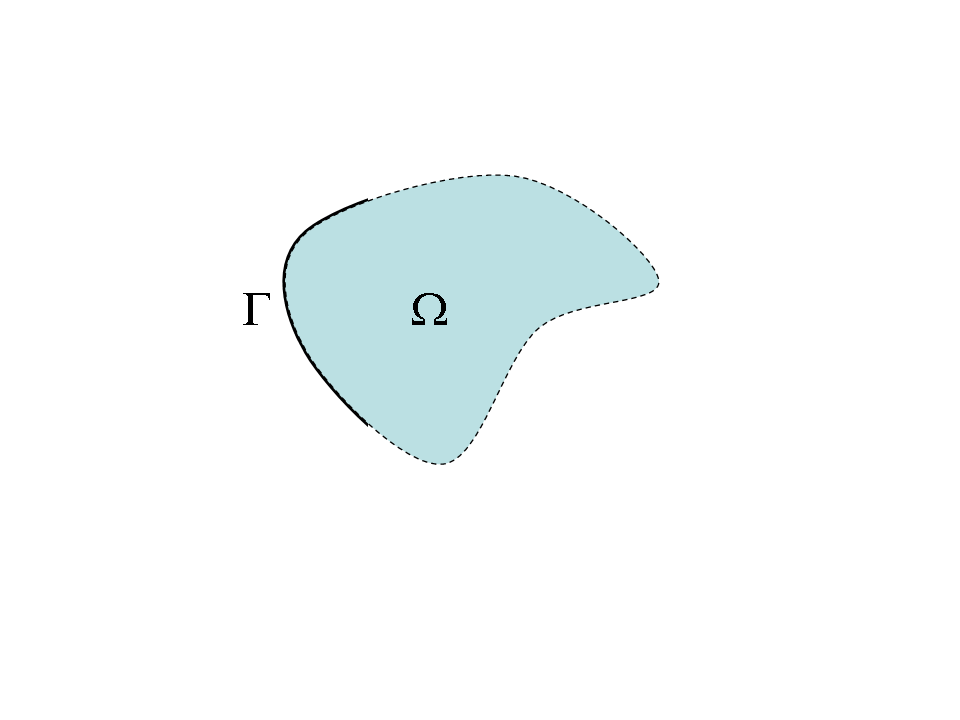
\includegraphics[width=0.6\textwidth]{domain}
\caption{Generic object being heated}\label{fg:domain}
\end{figure}  

At some part of the boundary the temperature is fixed.  Mathematically the problem is described by the Poisson equation
\begin{equation}
\left \{
\begin{array}{ccccc}
- \kappa \Delta T &= &\rho f & \mathrm{ in } \, \, & \Omega \\
T&=&0 & \mathrm{ on } & \Gamma
\end{array}
\right .
\end{equation}
where $\kappa$ is the heat conductivity, $T$  is the temperature and $f$ is the heat source. It is assumed that density and heat conductivity are constants. 

To determine the problem we assume that part of the boundary is fixed at $T_0=293$~K, the internal heat generation is, $h=0.01$~W/kg, and use the material properties of aluminium.  ElmerGUI has predefined values for many constants and material properties defined with SI units, so we will use SI units throughout this tutorial.  The goal of the simulation is to find out the temperature distribution in the object.


\subsection*{Existing Project}

The Elmer tutorials consist of the tutorial documentation and the tutorial folders.  For example, these ElmerGUI tutorials are described in the document 'ElmerTutorials.pdf' and the working project files are stored under the folder 'tutorials-GUI-files', and both can be downloaded from:  \url{https://www.nic.funet.fi/pub/sci/physics/elmer/doc/}

Each sub-folder under 'tutorials-GUI-files' contains all the files needed to run a particular tutorial, such as the ElmerGUI project file, the geometry input file, and the generated mesh files.  

If you wish to just run the existing project tutorial and examine the resulting output, start ElmerGUI and load the existing project file as follows:

\begin{verbatim}
File
  Load Project...
Run
  Start Solver
\end{verbatim}

You should see the Convergence Monitor and the Solver log windows pop up, and the solution finish in a few moments in most cases.  The results can then be examined using ElmerVTK or Paraview, as follow:

\begin{verbatim}
Run
  Start ElmerVTK
\end{verbatim}
or
\begin{verbatim}
Run
  Start Paraview
\end{verbatim}

\subsection*{New Project}

If you are more interested in learning how to use ElmerGUI by constructing an ElmerGUI project from the beginning, then the next few sections will describe in detail the step by step actions needed to build an ElmerGUI project.  The first step will be to create your own project folder, and copy in the geometry input file from the tutorial of interest.  Then start ElmerGUI and create a new project, as follows:

\begin{verbatim}
Run
  New Project...
\end{verbatim}

Start at the top and select the project directory as shown in Figure \ref{fg:new_project}.  Then select the Geometry input file, that was copied into your project folder.  This could either be an elmer mesh or a geometry input file, such as an elmergrid input file.  Lastly, if additional Equation Definition Files are needed for the tutorial, select as many as needed in the right hand box and add them to the left hand box.  Finish by clicking on OK.

\begin{figure}[H]
\centering
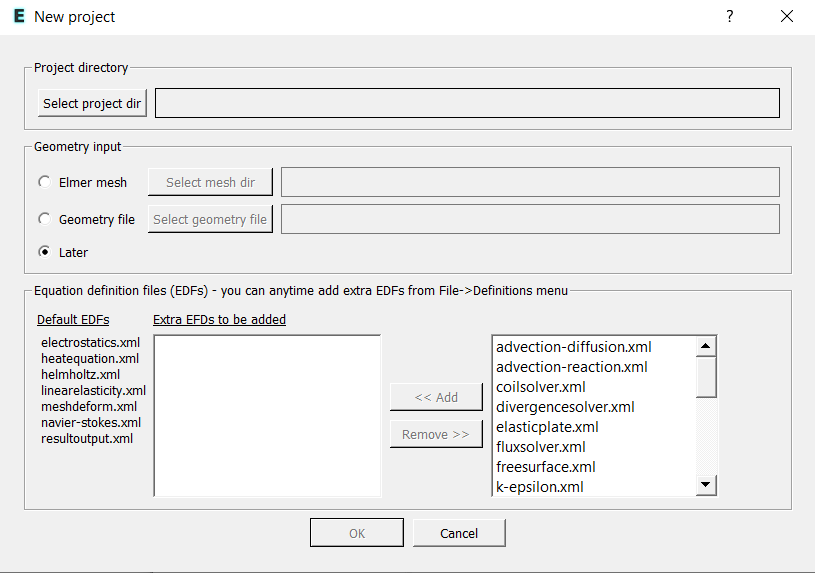
\includegraphics[width=0.8\textwidth]{new_project.png}
\caption{New Project}\label{fg:new_project}
\end{figure}  

\subsection*{ElmerGUI Equation Definition Files}

The New Project screen automatically locates and lists all of the available EDFs.  The left side of the screen lists the Default EDFs, which will be loaded into each ElmerGUI project.  The right hand box lists all of the extra EDFs, that are not normally loaded, allowing the option to add individual extra EDFs to a new project.\\

This tutorial will use the Default EDF, \texttt{\Idx{heatequation.xml}}, for the \Idx{Heat Solver}.

\subsection*{Solution procedure}

Start \texttt{ElmerGUI} from command line or by clicking the icon in your desktop. Here we describe the essential steps in the ElmerGUI by writing out the clicking procedure. Tabulation (indentation) generally means that the selections are done within the window chosen at the higher level. 

The geometry is given in step format in file \texttt{pump\_carter\_sup.stp} in the \texttt{samples/step} directory of ElmerGUI.  This file is kindly provided at the AIM@SHAPE Shape Repository by INRIA.  The heat equation is ideally suited for the finite element method and the solution may be found even at meshes that for some other problems would not be feasible. Therefore you may easily experiment solving the same problem with different meshes. If your particular version of ElmerGUI lacks OpenCascade, you might try to solve a similar problem with the \texttt{grd} files \texttt{angle3d.grd, angles3d.grd, bench.grd}, or \texttt{cooler.grd}, for example.

The CAD geometry defined by the step file is transformed on-the-fly by OpenCascade library into an stl file for which nglib creates tetrahedral volume discretization.  You may also use the tetlib library (tetgen) if you have installed it as a plug-in.

Load the input file:
\ttbegin
File 
  Open -> pump_carter_sup.stp
\ttend
The meshing will take a minute or two.  You should obtain your mesh and may check for the number of elements in the \texttt{Model summary}, as shown in Figure ~\ref{fg:mesh-default}.\\

\begin{figure}[H]
\begin{center}
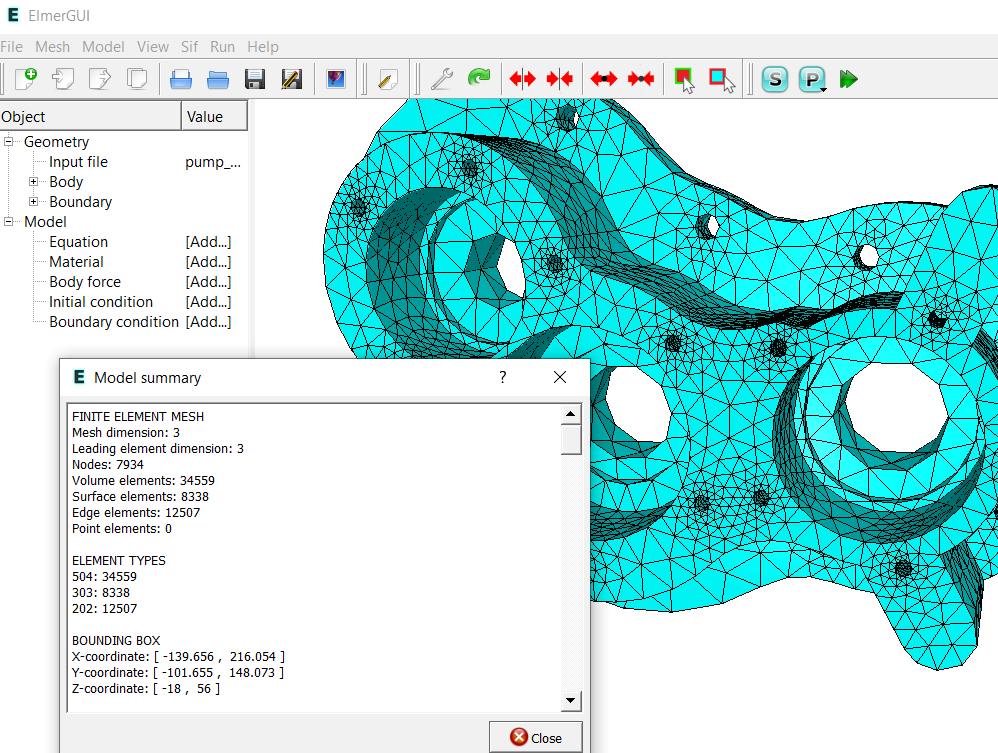
\includegraphics[width=0.90\textwidth]{mesh-default}
\caption{The computational mesh based on default settings}\label{fg:mesh-default}
\end{center}
\end{figure}

Visual inspection reveals that the mesh is not quite satisfactory in geometric accuracy.  We choose to modify the mesh by altering the settings in the following way, as shown in Figure ~\ref{fg:refinement}.  In order to affect the mesh density we set the maximum element size, max h, and the minimum element size, min h, and select the option to restrict mesh size on surfaces by the STL surface density.  Note that one must click on \texttt{Mesh, Remesh} in order for the new settings to be applied.\\

\begin{figure}[H]
\begin{center}
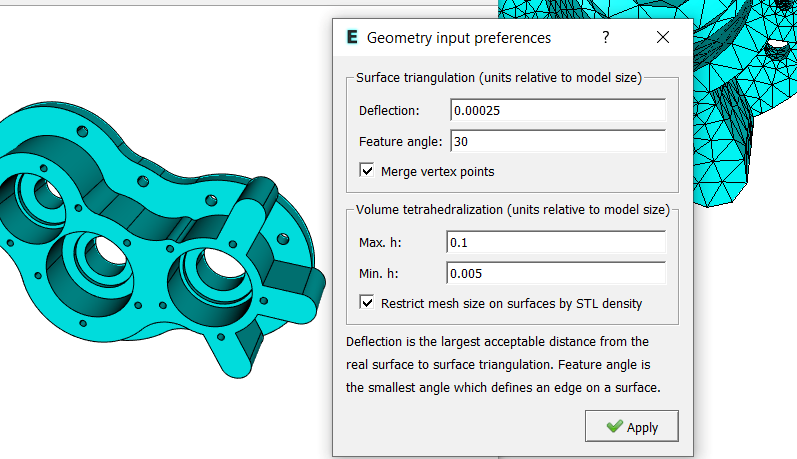
\includegraphics[width=0.80\textwidth]{refinement}
\caption{Refinement settings}\label{fg:refinement}
\end{center}
\end{figure}

\ttbegin
View -> Cad model...
  Model -> Preferences...
    Restrict mesh size on surfaces by STL density = on
    Apply
Mesh -> Remesh
\ttend

The meshing operation takes a minute or two.  The modified mesh should be more appealing to the eye. For example, notice the improvement in the inside diameters of the bores, they are more circular in shape.  You  may check for the number of elements in the \texttt{Model summary}, as shown in Figure ~\ref{fg:refinedmesh}.

Note that the remeshing operation will change the Elmer mesh.* files, but will not change the original geometry input file.  The   original step CAD file is unchanged, so any time the original geometry input file is input or reread, the meshing operations must be repeated.\\

\begin{figure}[H]
\begin{center}
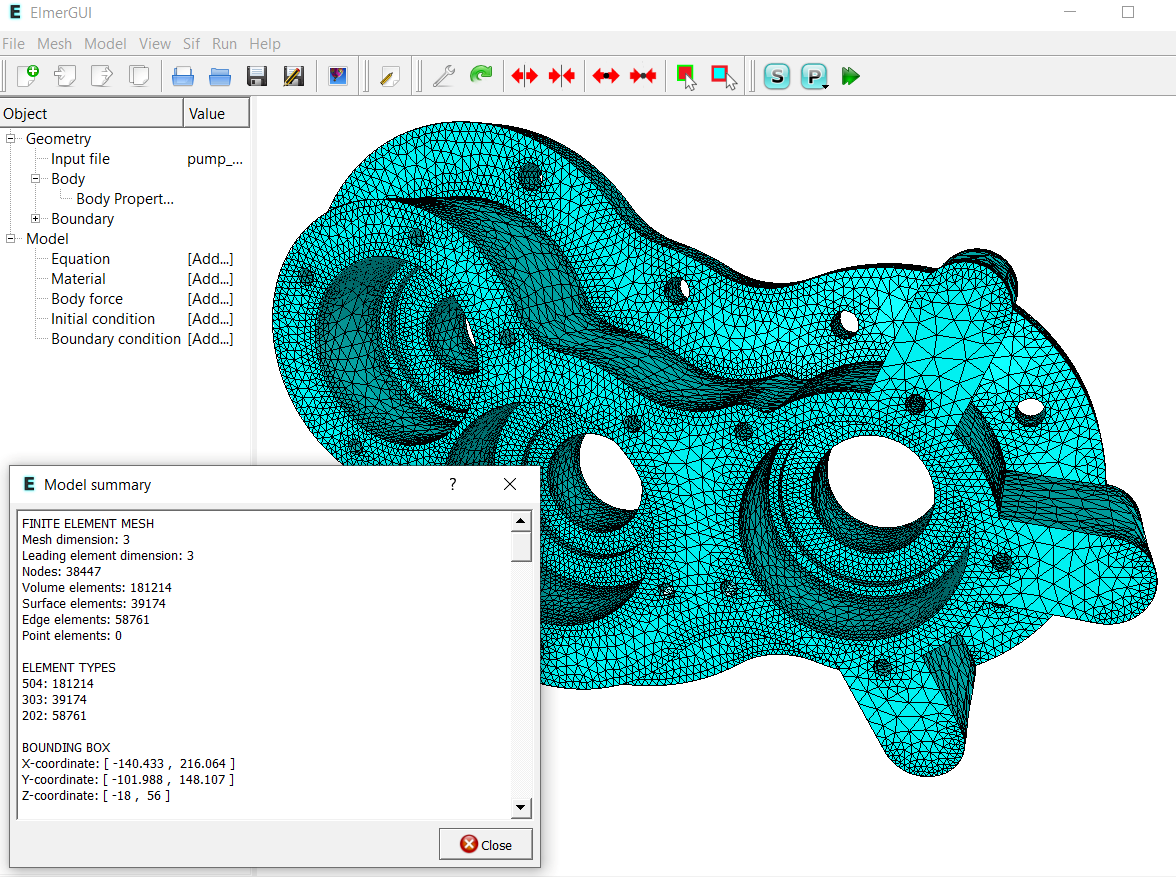
\includegraphics[width=0.90\textwidth]{refinedmesh}
\caption{Refined mesh}\label{fg:refinedmesh}
\end{center}
\end{figure}

We want to set the temperature at the inside of the three bores, each of which have two interior surfaces.  We could set the boundary conditions by selecting all six surfaces, one at a time, as shown in Figure~\ref{fg:select}.

ElmerGUI has the capability to join boundary surfaces, so that we can unite all six boundaries into a single boundary, which will make it easier to apply our boundary conditions for the simulation.  We demonstrate this optional step of 'Unify Surface' next.  Note that the Elmer mesh.* files will be updated with the changed boundary surfaces, and the original geometry input file will be unchanged.\\ 

\begin{figure}[H]
\begin{center}
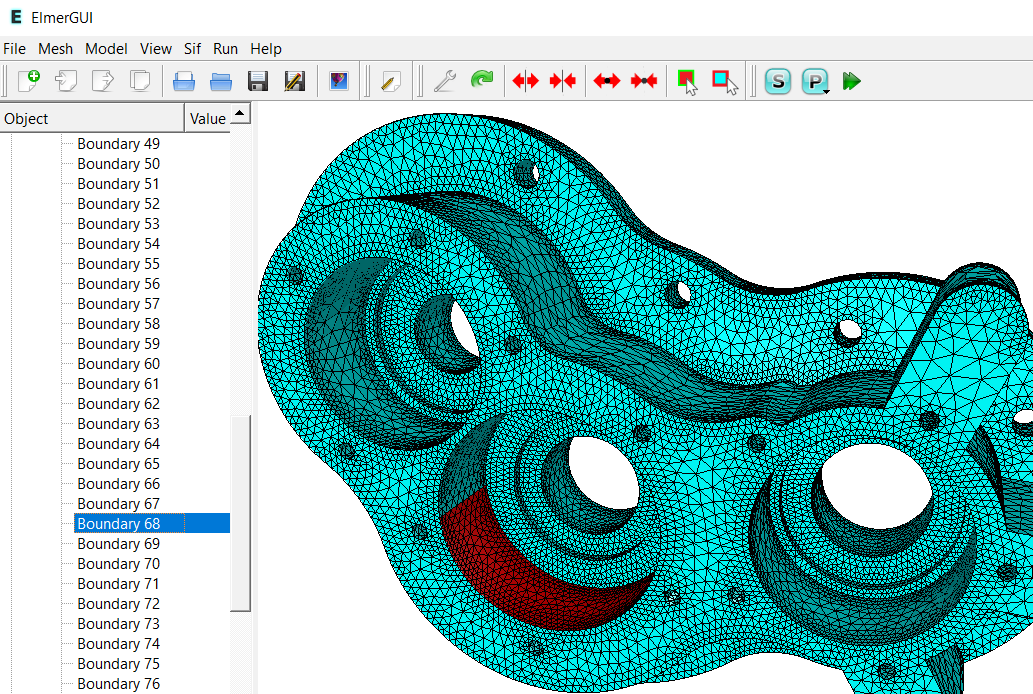
\includegraphics[width=0.8\textwidth]{select}
\caption{The computational mesh selecting one of the six interior boundaries}\label{fg:select}
\end{center}
\end{figure}

In order for ElmerGUI to unite surface boundaries, we must select the six pieces that constitute the boundaries.  Select the first surface by double clicking on the surface, then add the next five surfaces to the selection by double clicking while holding down the \texttt{Ctrl}-key.  Once all six surfaces are highlighted, use the menus to unify the surfaces.

\ttbegin
Mesh 
  Unify Surface
\ttend

\begin{figure}[H]
\begin{center}
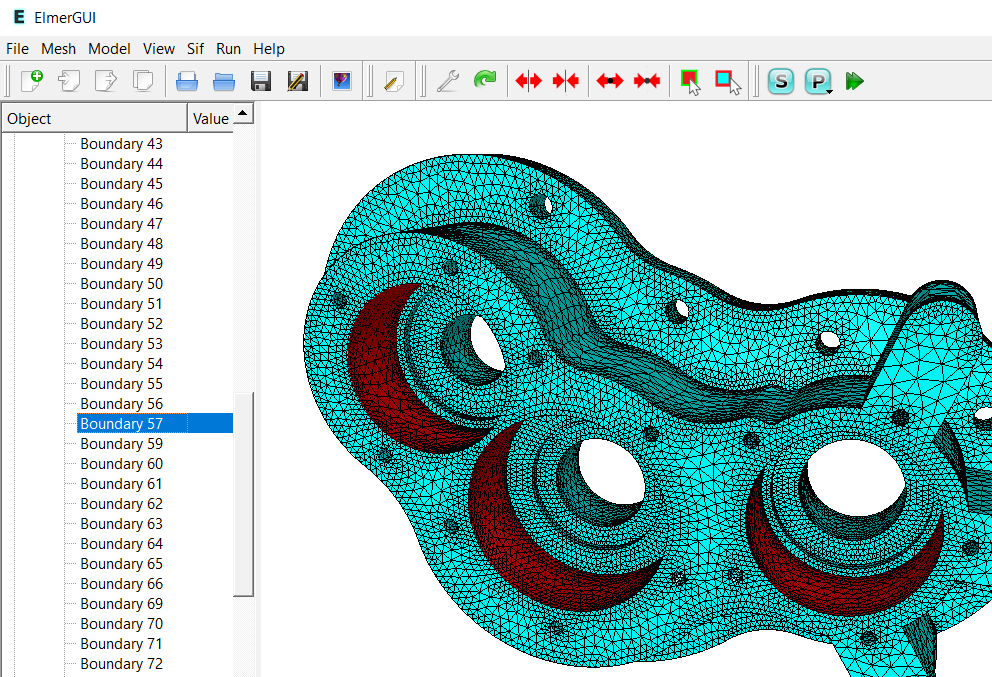
\includegraphics[width=0.8\textwidth]{bcs_chosen}
\caption{The computational mesh after uniting the six interior boundaries}\label{fg:bcs_chosen}
\end{center}
\end{figure}

After we have the mesh we start to go through the Model menu from the top to bottom.  The EDF menus include default settings for each entry, and we will highlight which particular entries should be set or changed.

In the \texttt{Setup} we choose things related to the whole simulation such as file names, time stepping, constants etc.  The simulation is carried out in 3-dimensional Cartesian coordinates and in steady-state.  Only one steady-state iteration is needed as the case is linear.

For this particular case, we can accept all of the default settings under Setup.  While the Setup window is open, take a look at all of the possible entries, as shown in Figure~\ref{fg:step-01}.  Note the two free text input boxes, one at the top and the other at the bottom.  Use the free text input boxes to add entries to the sif file such as comments about the model, or define constants, enter MATC commands, etc.

\ttbegin
Model
  Setup 
    Simulation Type = Steady state
    Steady state max. iter = 1
\ttend
Choose \texttt{Apply} to close the window.

\begin{figure}[H]
\begin{center}
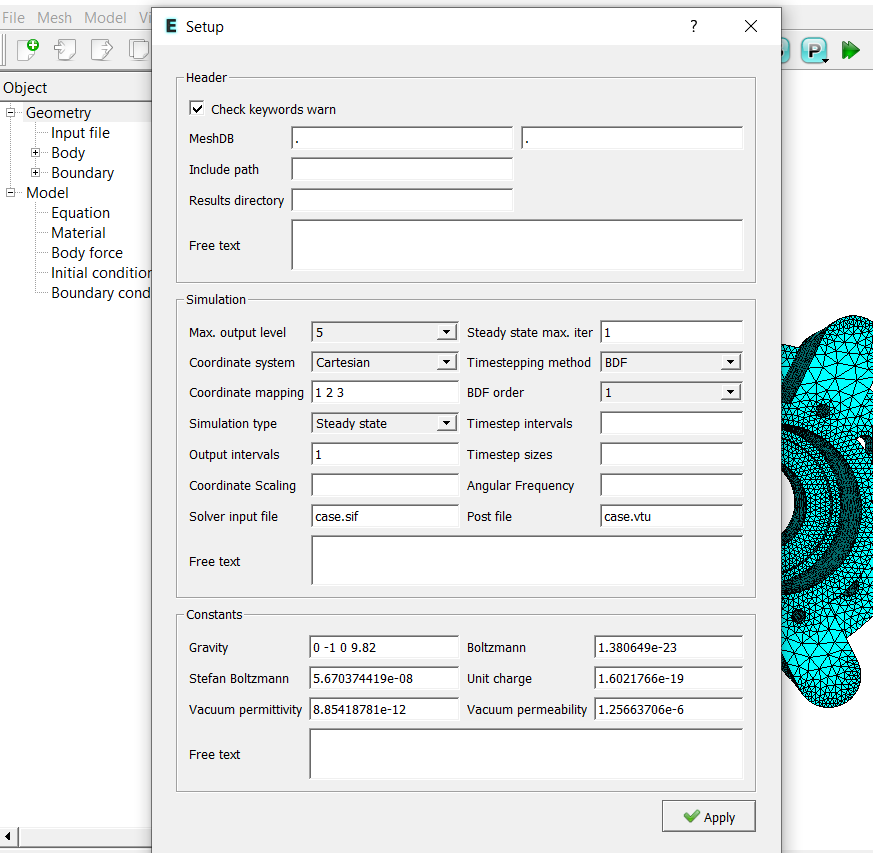
\includegraphics[width=0.8\textwidth]{step-01}
\caption{The Setup window}\label{fg:step-01}
\end{center}
\end{figure}

In the equation section we choose the relevant equations and parameters related to their solution.  In this case we'll have one set only one equation -- the heat equation, as shown in Figure~\ref{fg:step-02}.

When defining Equations and Materials it is possible to assign to the bodies immediately, or to use mouse selection to assign them later. In this case we have just one body and therefore it is easier to assign the Equation and Material to the body directly, whereas the active boundary is chosen graphically.

\ttbegin
Model
  Equation
    Add 
      Heat Equation
        Active = on
      Apply to bodies = Body 1
      Name = Heat Equation
      Add   
      OK
\ttend        

For the linear system solvers we are happy to use the defaults.  Click on  \texttt{Edit Solver Settings} to review the possible settings.  One may however, try out different preconditioners (ILU1,\ldots), for example.

\begin{figure}[H]
\begin{center}
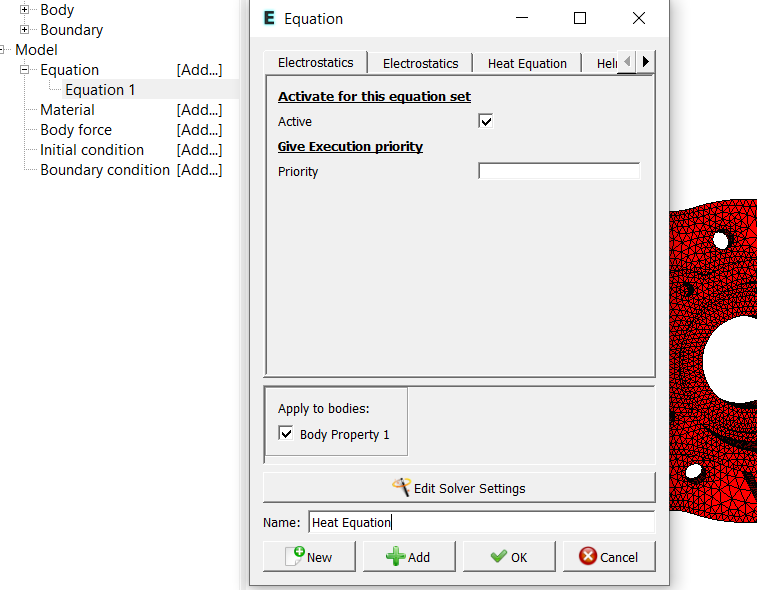
\includegraphics[width=0.8\textwidth]{step-02}
\caption{The Equation window}\label{fg:step-02}
\end{center}
\end{figure}

The Material section includes all the material parameters.  The tabs near the top for each equation are divided to generic parameters which are direct properties of the material without making any assumptions on the physical model, such as the mass. Other properties assume a physical law, such as heat conductivity.  We choose Aluminium from the Material library which automatically sets the needed material properties.

\ttbegin
Model
  Material
    Add 
      Apply to bodies = Body 1 
      Material library
        Aluminium (generic)
      Add 
      OK
\ttend

Click on the tabs near the top of the window, such as 'General' or 'Heat Equation', to inspect the values set by selecting the predefined material from the Material Library, as shown in Figure~\ref{fg:step-03}.

\begin{figure}[H]
\begin{center}
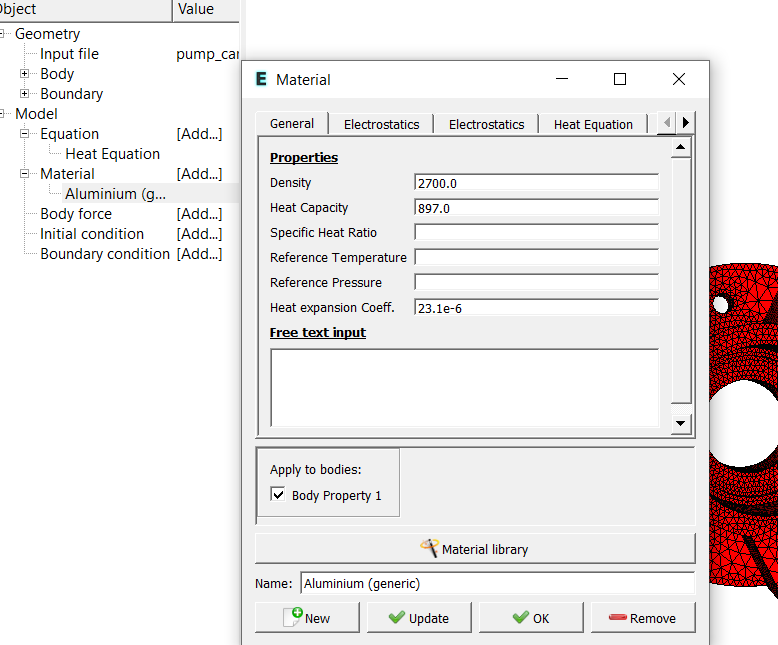
\includegraphics[width=0.8\textwidth]{step-03}
\caption{The Material window, showing the General tab}\label{fg:step-03}
\end{center}
\end{figure}

A Body Force represents the right-hand-side of a equation that in this case represents the heat source. 
\ttbegin
Model
  Body Force
    Add 
      Heat Equation
        Heat Source = 0.01
      Apply to bodies = Body 1
      Name = Heating
      Add
      OK
\ttend

Click on the tabs near the top of the window, to show the 'Heat Equation' tab, and inspect the possible values, as shown in Figure~\ref{fg:step-04}.

\begin{figure}[H]
\begin{center}
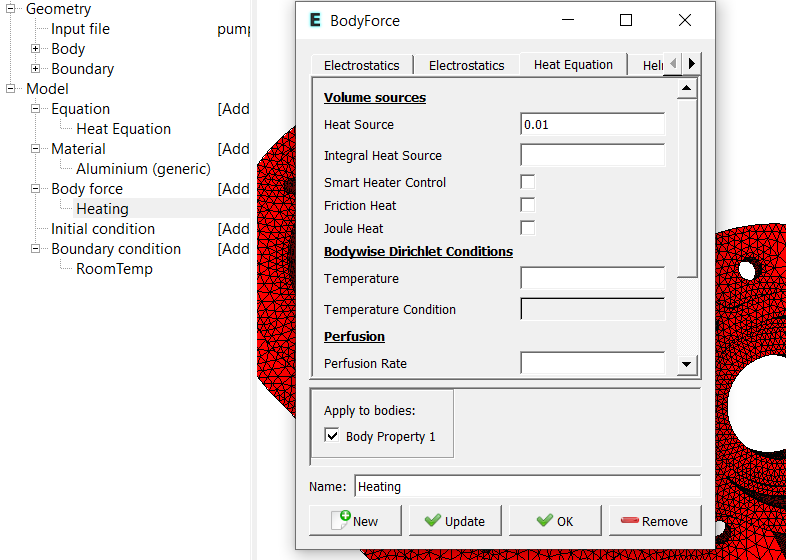
\includegraphics[width=0.8\textwidth]{step-04}
\caption{The Body Force window, showing the Heat Equation tab}\label{fg:step-04}
\end{center}
\end{figure}

No initial conditions are required in a steady state case.  Initial conditions are usually only needed for transient studies.  Note that the default temperature setting for any model is zero, which doesn't affect a steady state study, but will be important for a transient study.  The Initial Condition input window is similar to the Body Force window, as shown in Figure~\ref{fg:step-05}.\\

\begin{figure}[H]
\begin{center}
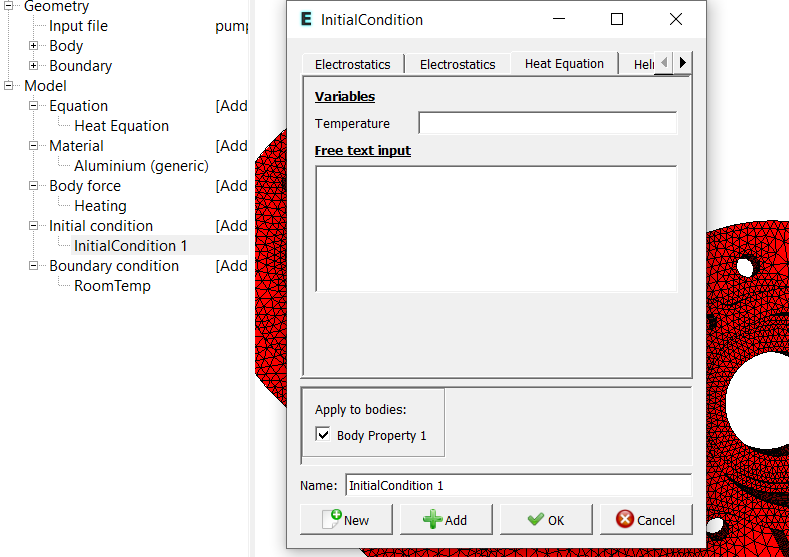
\includegraphics[width=0.8\textwidth]{step-05}
\caption{The Initial Condition window, showing the Heat Equation tab}\label{fg:step-05}
\end{center}
\end{figure}

In this case we will set only one boundary condition, which will be a fixed surface temperature, set to room temperature.  You may have noticed that there are many surface boundaries listed for the geometry, as previously shown in Figure~\ref{fg:select}.  For the heat equation, the default boundary condition is zero heat flux, or fully insulated, and for this example case we don't need to create boundary conditions for the other surfaces.\\

First we create the boundary condition, as shown in Figure~\ref{fg:step-06}.  Note that we do not assign the new boundary condition to any particular boundary, that assignment will happen when we set the boundary properties.

\ttbegin
Model
  BoundaryCondition
    Add 
      Heat Equation
        Temperature = 293.0
      Name = RoomTemp
      Add
      OK
\ttend   

\begin{figure}[H]
\begin{center}
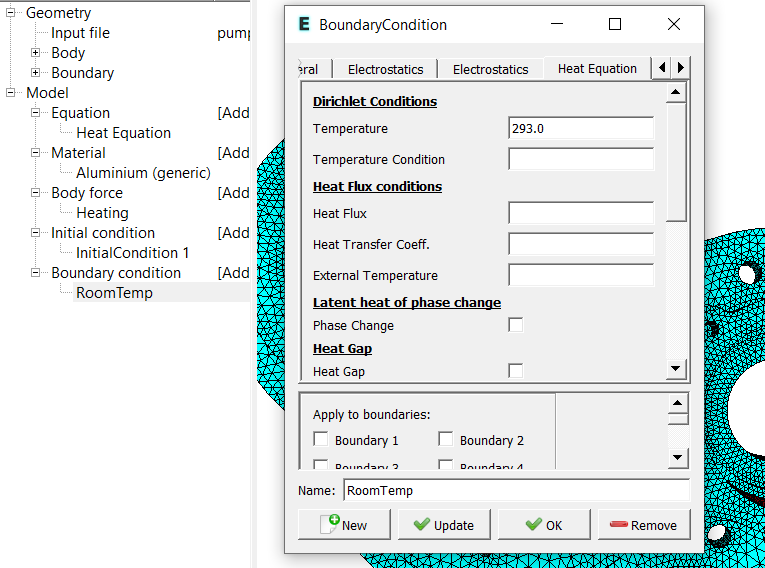
\includegraphics[width=0.8\textwidth]{step-06}
\caption{The Boundary condition window}\label{fg:step-06}
\end{center}
\end{figure}

Then we set the boundary properties, as shown in Figure~\ref{fg:step-07}.  Select our desired boundaries and then assign a boundary condition to those boundaries.

\ttbegin
Model 
  Set boundary properties  
\ttend

\begin{figure}[H]
\begin{center}
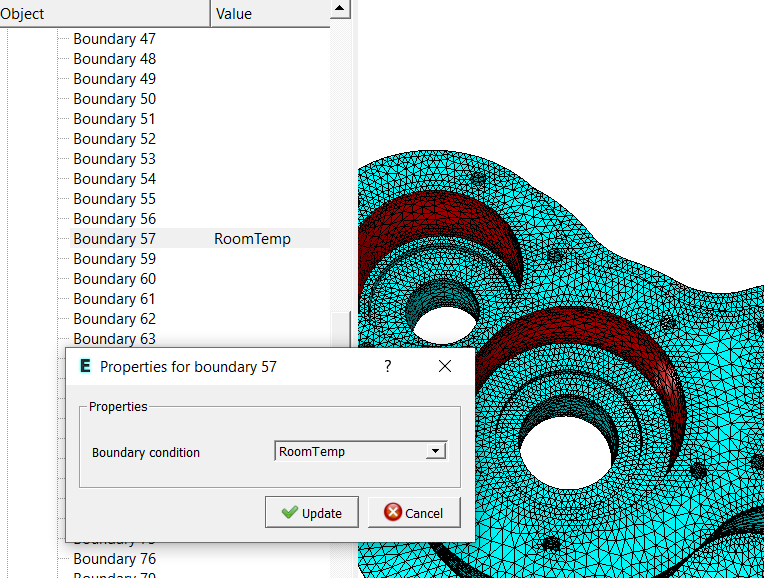
\includegraphics[width=0.7\textwidth]{step-07}
\caption{The Boundary property window}\label{fg:step-07}
\end{center}
\end{figure}

For our case, we will select the united group of three interior bores by double clicking with the mouse and then apply the condition for this boundary.
\ttbegin
Boundary condition
  RoomTemp
\ttend

For the execution of the simulation, ElmerSolver needs the mesh files and the sif command file. We have now basically defined all the information for ElmerGUI to write the command file.\\

\ttbegin
Sif 
  Generate
  Edit -> look how your command file came out  
\ttend

After writing the sif file, we may also visually inspect, and optionally edit, the command file, as shown in Figure~\ref{fg:step-08}.

\begin{figure}[H]
\begin{center}
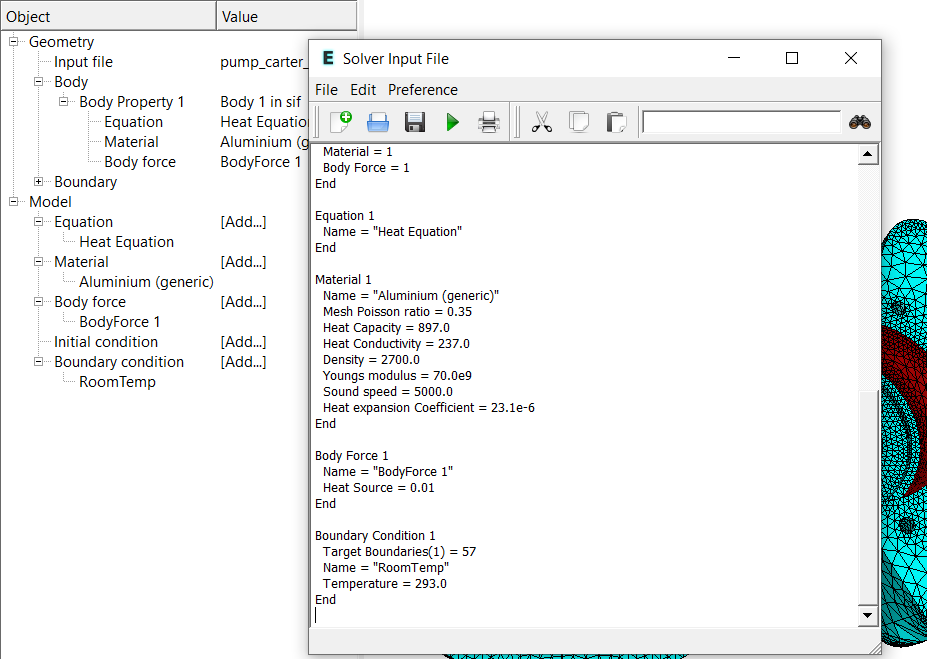
\includegraphics[width=0.8\textwidth]{step-08}
\caption{The Sif editor window}\label{fg:step-08}
\end{center}
\end{figure}

Before we can execute the solver we should save the files in a directory. In saving the project all the necessary files for restarting the case will be saved to the destination directory.
\ttbegin
File 
  Save Project
\ttend

After we have successfully saved the files we may start the solver
\ttbegin
Run
  Start solver
\ttend
The solver log and a convergence view automatically pops up showing relative changes of each iteration, as shown in Figure~\ref{fg:step-09}.  

\begin{figure}[H]
\begin{center}
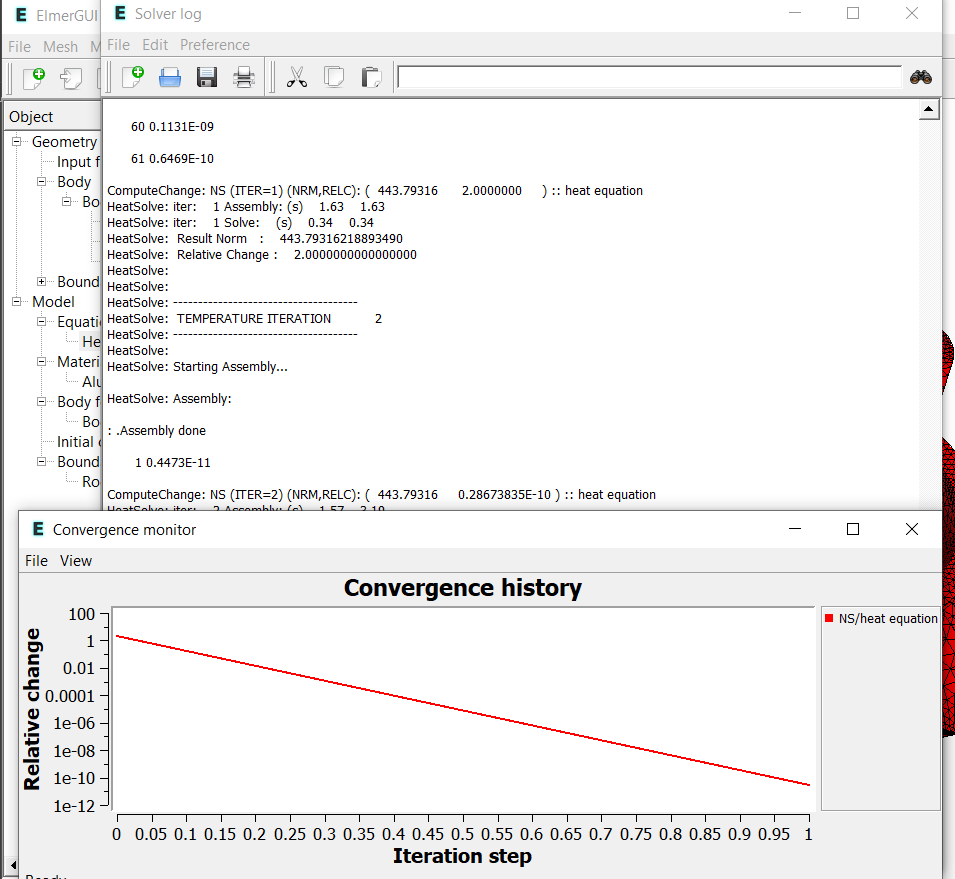
\includegraphics[width=0.8\textwidth]{step-09}
\caption{The Solver log and convergence windows}\label{fg:step-09}
\end{center}
\end{figure}

As the case is linear only one iteration was required for the solution and the second one just is needed to check the convergence. The norm of the solution should be around 432.4~K (with the default tetgen mesh 389.8~K, respectively).

Note: if you face problems in the solution phase and need to edit the settings, always remember to regenerate the sif file and save the project before execution.

Once one gets used to generating sif files and running the solver, ElmerGUI includes a double green arrow icon.  The double green arrow icon combines all three steps into a single mouse click:\\
\texttt{Generate and save sif, save project, and then run solver.}

\subsection*{Postprocessing with ElmerVTK}

\Idx{ElmerVTK} is a simple post processor to use, and makes sense for a first look at Elmer simulation results.  We will cover Paraview later, which is a more powerful visualization program and, of course, is also a little harder to learn and use.\\

To view the results we will run ElmerVTK for the visualization.

\ttbegin
Run
  ElmerVTK
\ttend

\newpage
The initial window for ElmerVTK will pop up, with the surface of the geometry colored in blue, as shown in Figure~\ref{fg:vtk-1}.  Observe the row of tabs along the top of the window.  To hide the surface coloring, left click on the \texttt{Surfaces} tab.

\begin{figure}[H]
\begin{center}
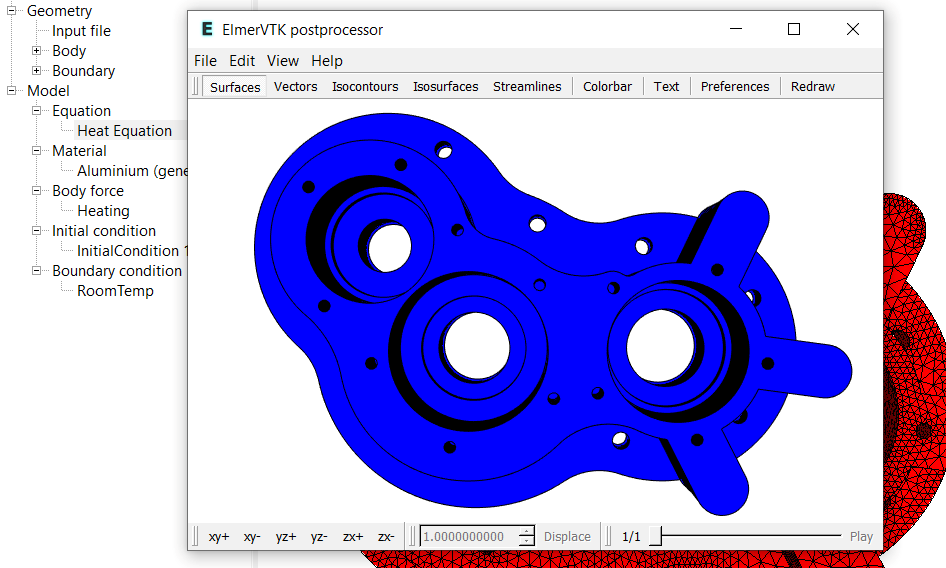
\includegraphics[width=0.8\textwidth]{vtk-1}
\caption{The ElmerVTK window, Surfaces}\label{fg:vtk-1}
\end{center}
\end{figure}

We want to add 3D contouring, so click on the \texttt{Isosurfaces} tab.  Click in the Contour control Variable box, and select temperature from the drop down box.  Continue and click in the Color control Color drop box and again select temperature, as shown in Figure~\ref{fg:vtk-2}.

\begin{figure}[H]
\begin{center}
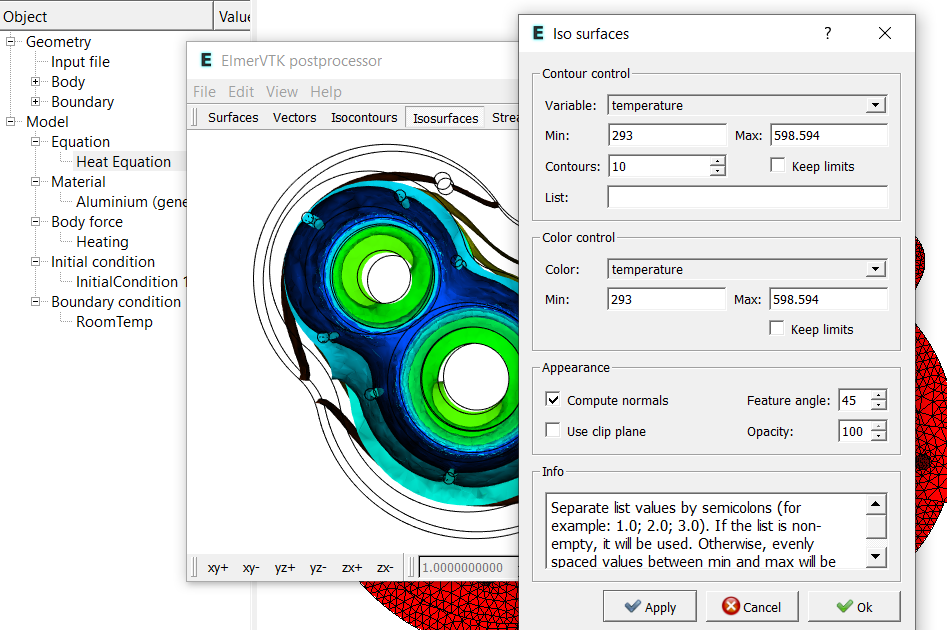
\includegraphics[width=0.8\textwidth]{vtk-2}
\caption{The ElmerVTK window, Isosurfaces selection}\label{fg:vtk-2}
\end{center}
\end{figure}

Click on Apply and Ok, to apply the settings and close the pop up selection window.

\newpage

The isosurfaces will be displayed, as shown in Figure~\ref{fg:vtk-3}.  Use the mouse to rotate the part, to see the isosurfaces from different viewpoints.

\begin{figure}[H]
\begin{center}
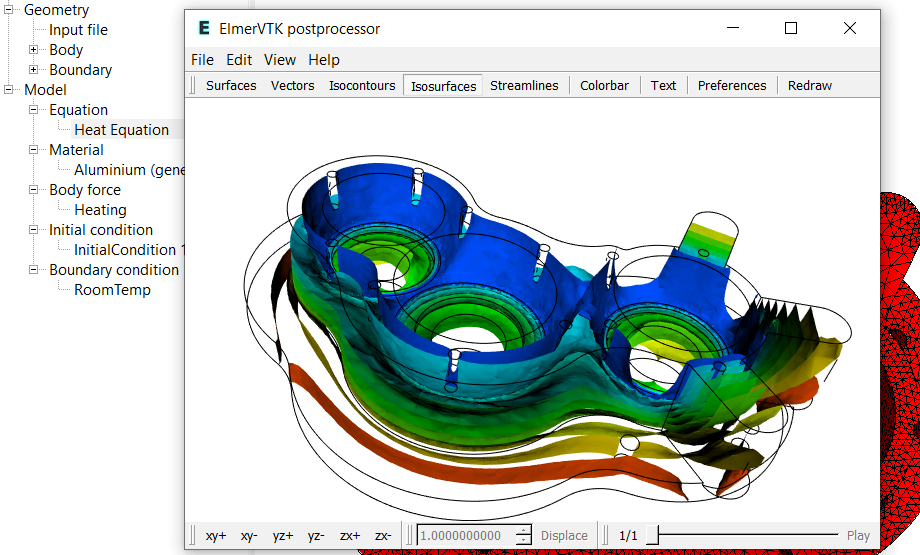
\includegraphics[width=0.8\textwidth]{vtk-3}
\caption{The ElmerVTK window, Isosurfaces shown}\label{fg:vtk-3}
\end{center}
\end{figure}

Let's add a color bar to the view, so we can see the range of temperatures in the simulation.  Click on the \texttt{Colorbar} tab.  The Colorbar selection menu will pop up, as shown in Figure~\ref{fg:vtk-4}.  Click in the Color map drop box, and select Isosurface.  Also, click on the radio button for Vertical, to locate the color bar along the left side.

\begin{figure}[H]
\begin{center}
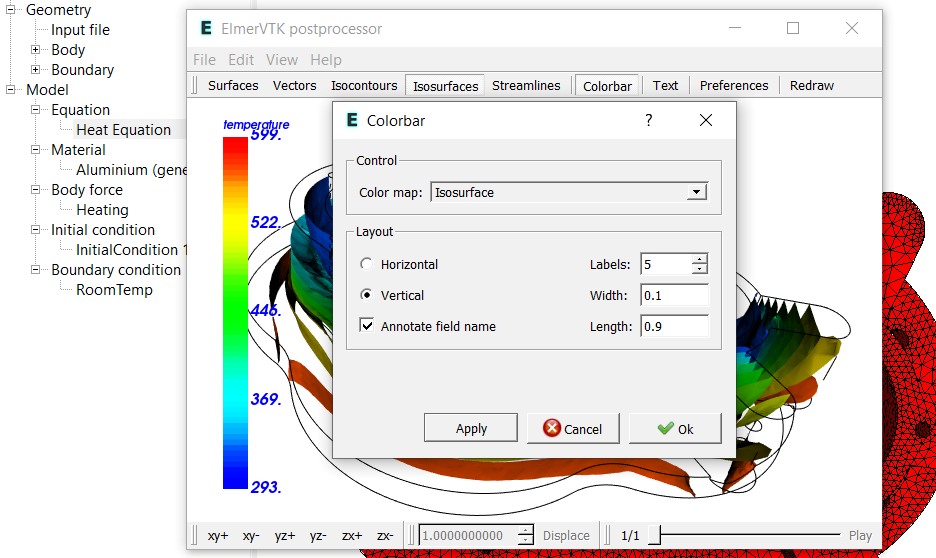
\includegraphics[width=0.8\textwidth]{vtk-4}
\caption{The ElmerVTK window, Colorbar selection}\label{fg:vtk-4}
\end{center}
\end{figure}

Click on Apply and Ok, to apply the settings and close the pop up selection window.

\newpage

The color bar and the isosurfaces will be displayed, as shown in Figure~\ref{fg:vtk-5}.

\begin{figure}[H]
\begin{center}
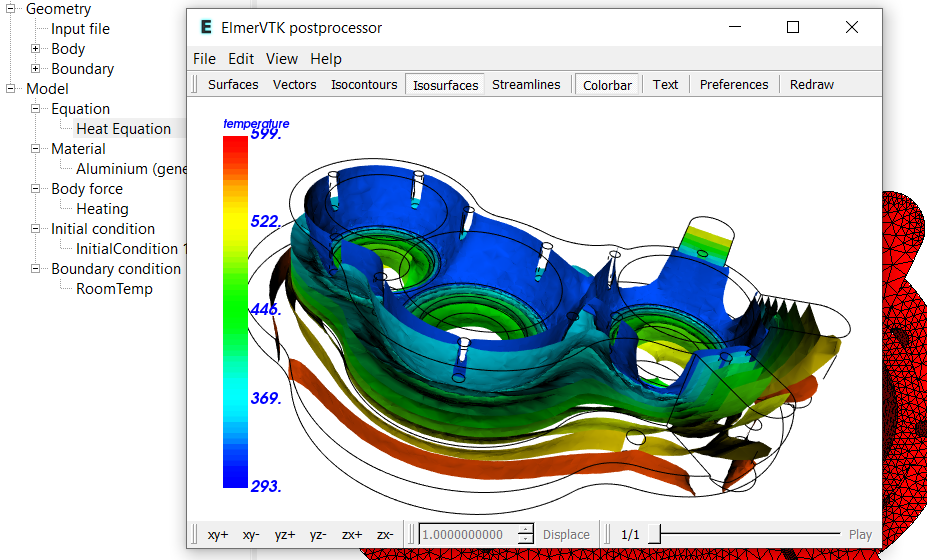
\includegraphics[width=0.8\textwidth]{vtk-5}
\caption{The ElmerVTK window, with color bar}\label{fg:vtk-5}
\end{center}
\end{figure}

To demonstrate how to \Idx{save a picture with ElmerVTK}, click on \texttt{File, Save picture as}, then select a file name and directory to store the picture, and ElmerVTK will save your simulation results, as shown in Figure~\ref{fg:vtk-6}.  If the picture is too small or too large for you, just resize the ElmerVTK window and save the picture again.

\begin{figure}[H]
\begin{center}
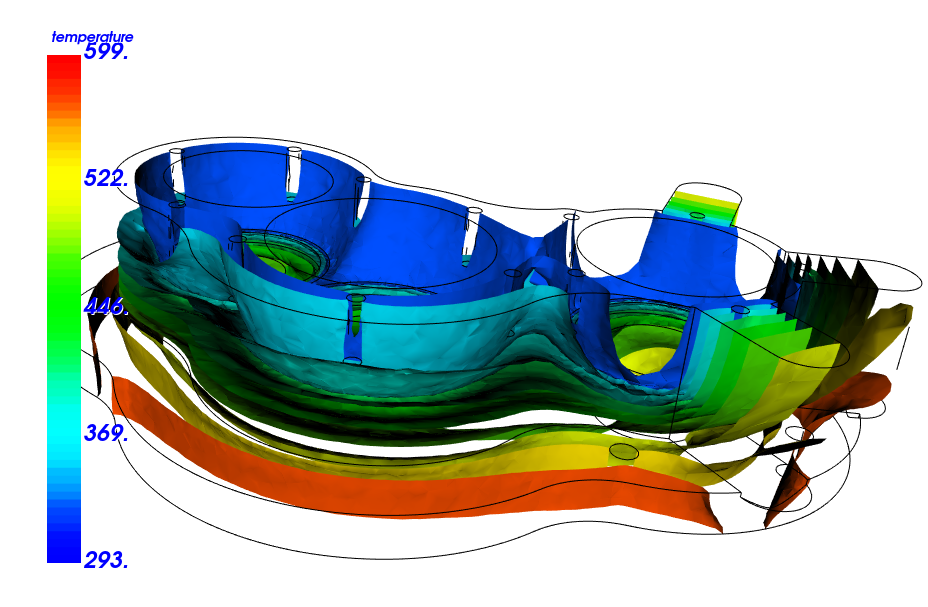
\includegraphics[width=0.8\textwidth]{vtk-6}
\caption{The ElmerVTK window, final results}\label{fg:vtk-6}
\end{center}
\end{figure}

\newpage

Next we will demonstrate \Idx{clipping with ElmerVTK}, which may be very helpful for 3D simulations.  Refer back to the Isosurfaces selection window in Figure~\ref{fg:vtk-2}, under the section \texttt{Appearances}, click on \texttt{Use clip plane}, and then \texttt{Apply}.  The results are shown in Figure~\ref{fg:vtk-7}.

\begin{figure}[H]
\begin{center}
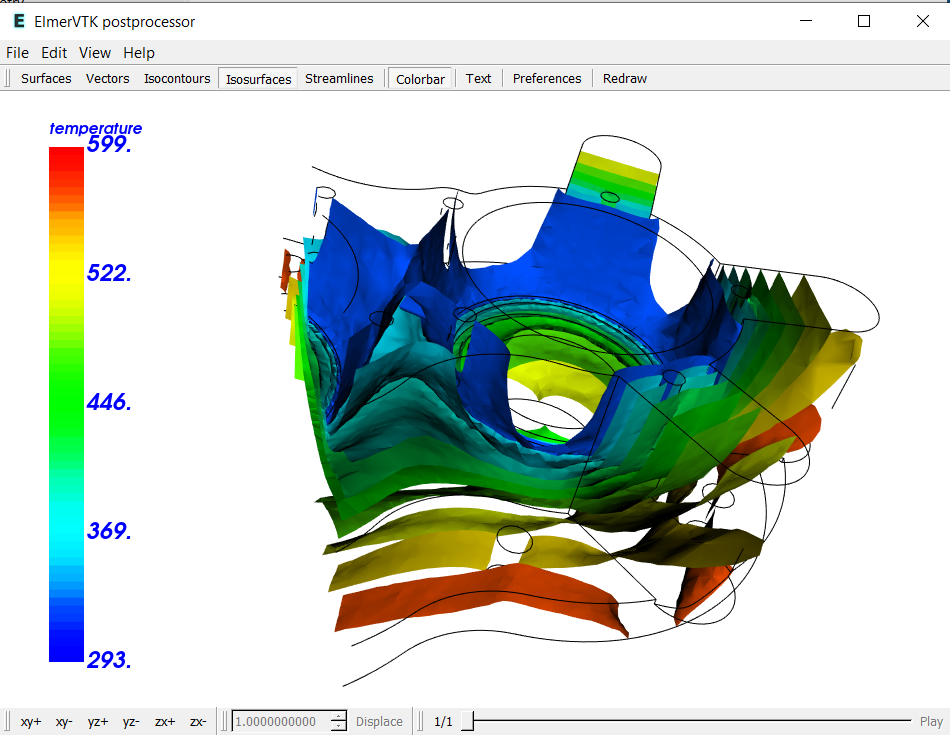
\includegraphics[width=0.6\textwidth]{vtk-7}
\caption{The ElmerVTK window, clip plane applied}\label{fg:vtk-7}
\end{center}
\end{figure}

ElmerGUI supplies a default clip plane setting going in the X direction, through the center of the model.  To adjust the clip plane settings, click on the tab \texttt{Preferences}, and notice at the bottom are six settings.  Adjust the X, Y, or Z coordinates, or adjust the X, Y, or Z normals.  Note that one may use a negative normal, such as -1, to clip the model in the opposite direction.

\begin{figure}[H]
\begin{center}
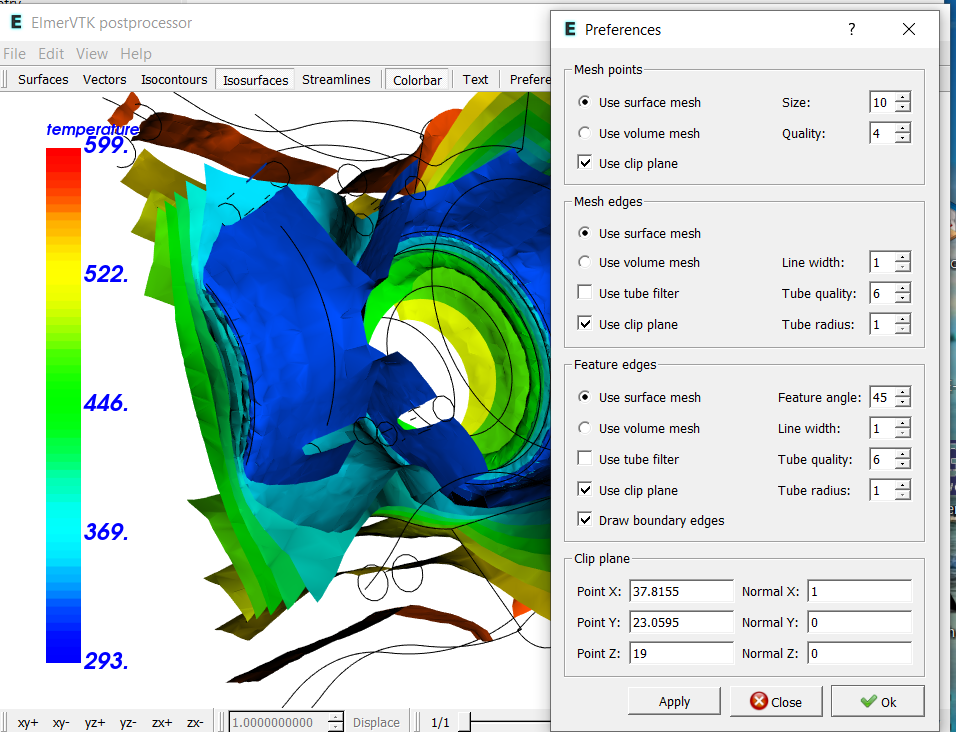
\includegraphics[width=0.6\textwidth]{vtk-8}
\caption{The ElmerVTK window, Preferences and clip plane}\label{fg:vtk-8}
\end{center}
\end{figure}

One can now close ElmerVTK, or spend some time exploring a few more features of ElmerVTK, such as Vectors.  Also, if one runs a transient study, ElmerVTK can show each of the time steps, using the slider control at the bottom right of the window.

\subsection*{Postprocessing with Paraview}

Next we will cover the basics of using \Idx{Paraview} to visualize the simulation results.

\ttbegin
Run
  Paraview
\ttend

After a short wait, Paraview will open and it should show our case\_t0001.vtu file in the upper left window, as shown in Figure~\ref{fg:paraview-1}.  First step is to click on the light green Apply button.

\begin{figure}[H]
\begin{center}
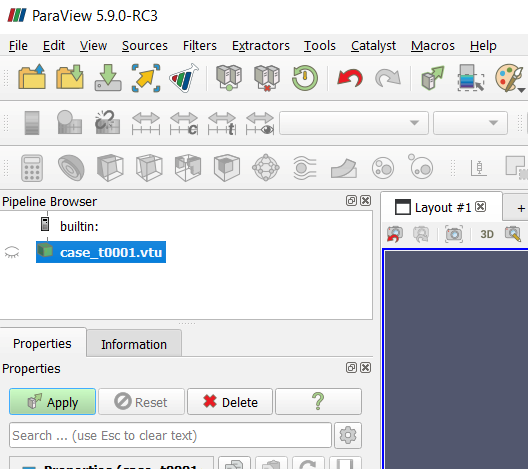
\includegraphics[width=0.5\textwidth]{paraview-1}
\caption{The Paraview window, click on Apply}\label{fg:paraview-1}
\end{center}
\end{figure}

Once we have clicked on Apply, the geometry will appear in the layout port, and will be all grey.  We will then tell Paraview which simulation results we wish to display, by clicking on the  button under the section header \texttt{Coloring} located in the lower left corner, as shown in Figure~\ref{fg:paraview-2}.  Select temperature in the drop box, as shown in Figure~\ref{fg:paraview-2}.

\begin{figure}[H]
\begin{center}
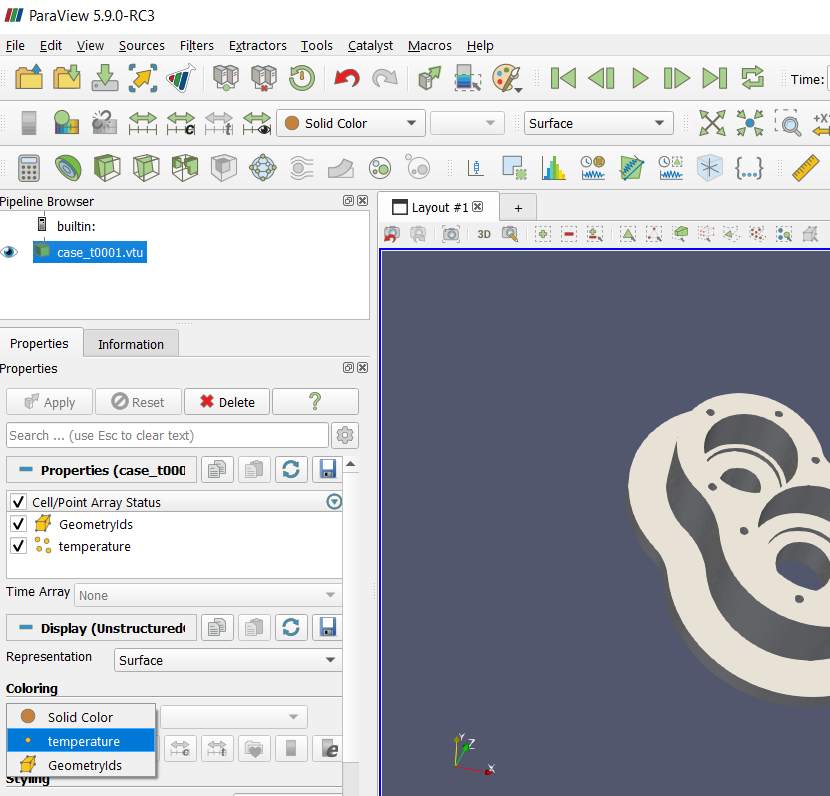
\includegraphics[width=0.5\textwidth]{paraview-2}
\caption{The Paraview window, select variable}\label{fg:paraview-2}
\end{center}
\end{figure}

The temperature of the simulation will be displayed in the layout port, along with a color bar that is automatically added to the layout, as shown in Figure~\ref{fg:paraview-3}.

\begin{figure}[H]
\begin{center}
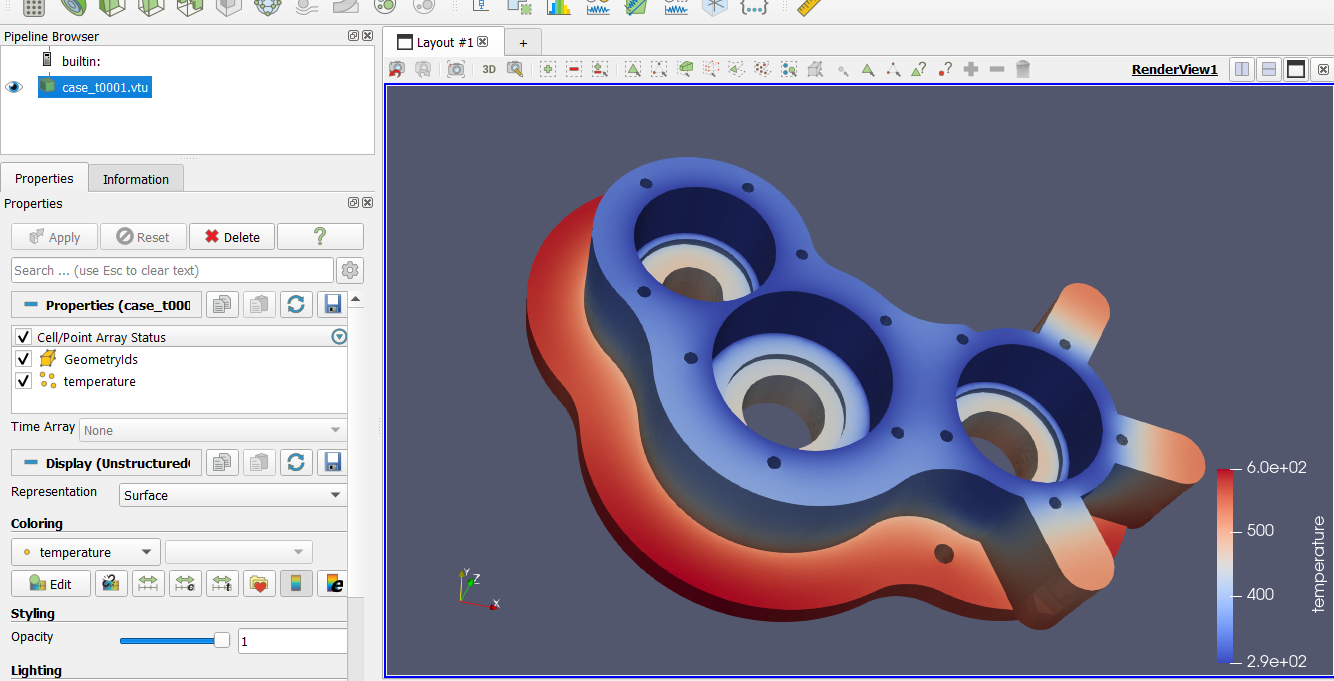
\includegraphics[width=0.95\textwidth]{paraview-3}
\caption{The Paraview window, showing results}\label{fg:paraview-3}
\end{center}
\end{figure}

Lastly, let's \Idx{save a picture with Paraview}.  At the top of the window, click on \texttt{File}, then  \texttt{Save Screenshot}, as shown in Figure~\ref{fg:paraview-4}.

\begin{figure}[H]
\begin{center}
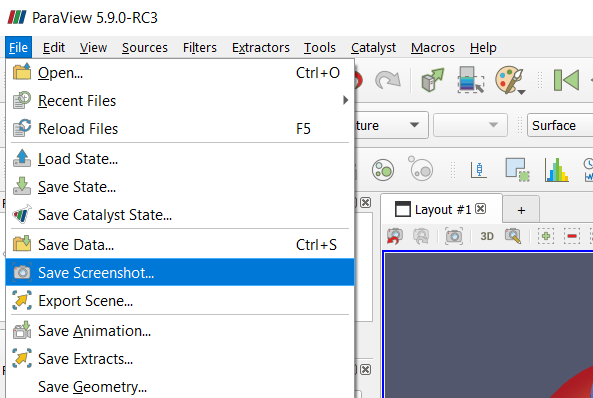
\includegraphics[width=0.7\textwidth]{paraview-4}
\caption{The Paraview window, Screenshot}\label{fg:paraview-4}
\end{center}
\end{figure}

\newpage

Follow the prompts, such as selecting a file name and directory to store the picture, select the size in pixels of the picture, and Paraview will save your simulation results, as shown in Figure~\ref{fg:paraview-5}.

\begin{figure}[H]
\begin{center}
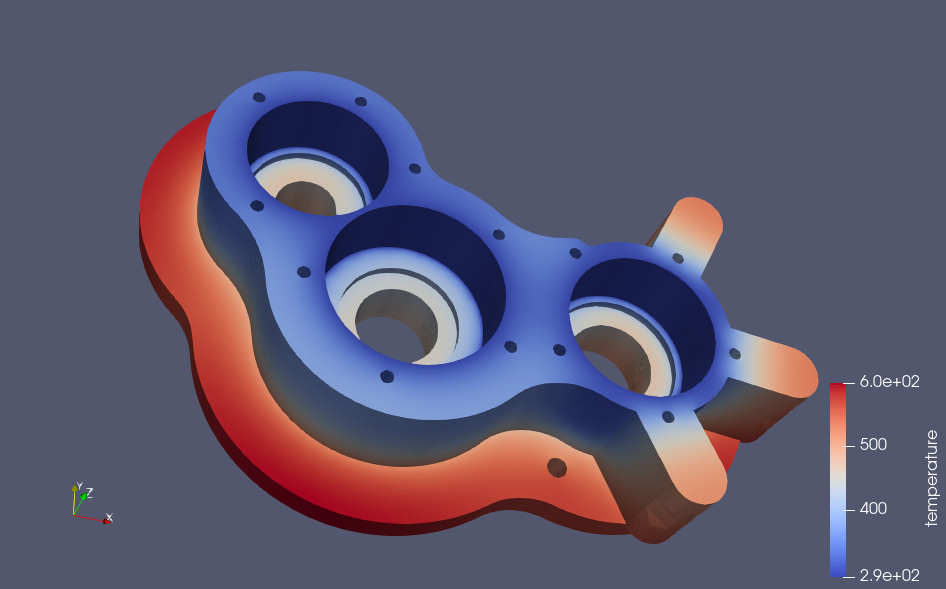
\includegraphics[width=0.95\textwidth]{paraview-5}
\caption{The Paraview window, final results}\label{fg:paraview-5}
\end{center}
\end{figure}

Paraview has many options, as you can see from the many icons in the main window.  As one example, we will demonstrate \Idx{clipping with Paraview}, which may be very helpful for 3D simulations.  At the top bar, click on \texttt{Filters, Common, Clip}, as shown in Figure~\ref{fg:paraview-6}.  As always with Paraview, click on the light green Apply button to apply the action to the layout.

\begin{figure}[H]
\begin{center}
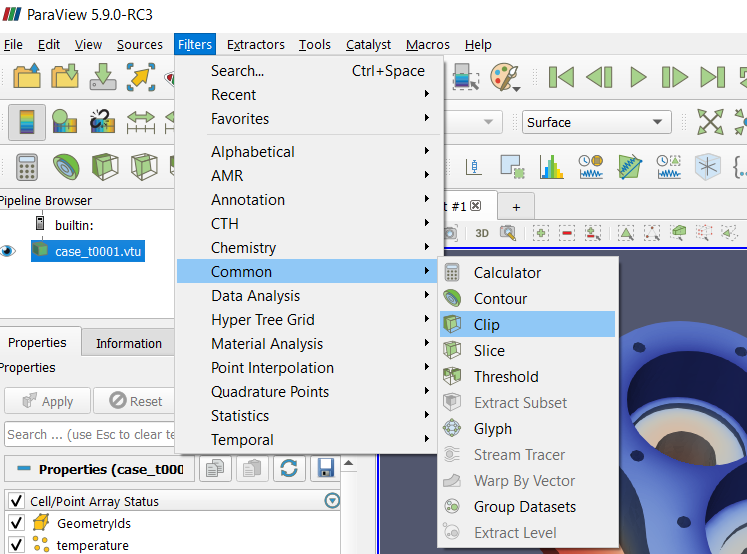
\includegraphics[width=0.7\textwidth]{paraview-6}
\caption{The Paraview window, Filter, Common, Clip}\label{fg:paraview-6}
\end{center}
\end{figure}

\newpage

One can rotate the model, along with moving the clip plane, or selecting direction with X, Y, or Z normals.  These steps will be left to the student to discover.

\begin{figure}[H]
\begin{center}
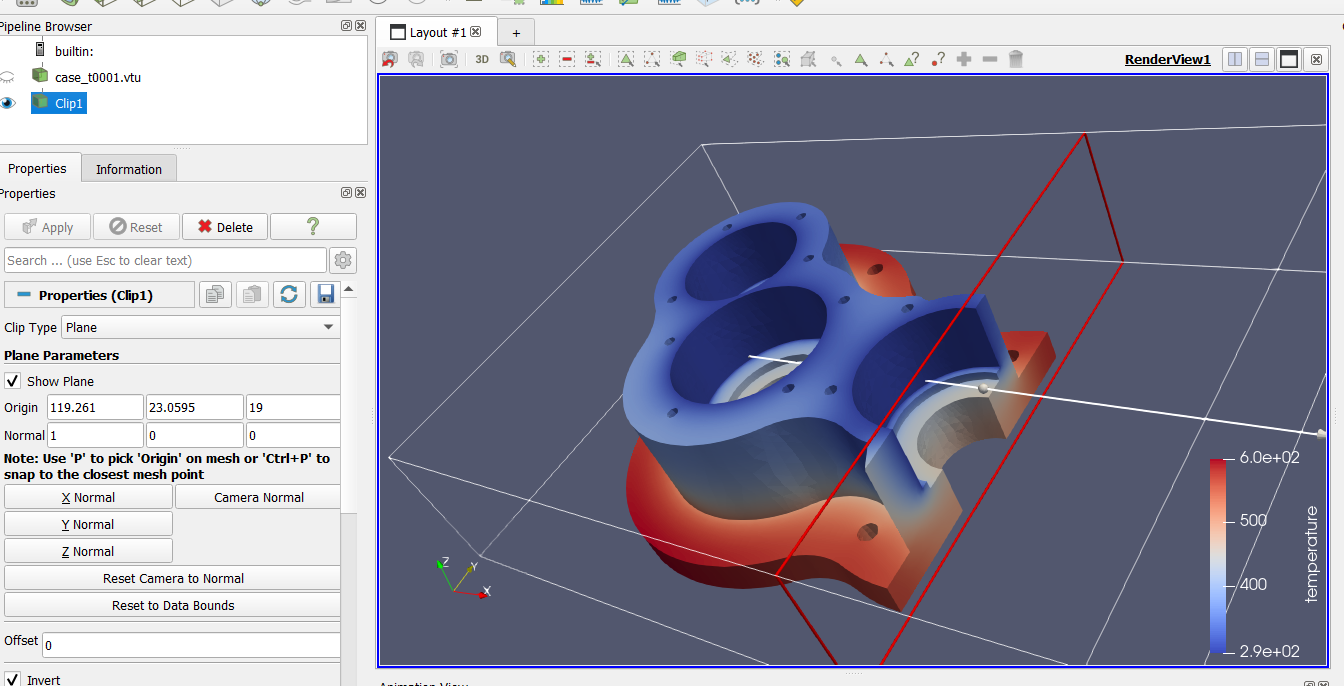
\includegraphics[width=0.95\textwidth]{paraview-7}
\caption{The Paraview window, clipped results}\label{fg:paraview-7}
\end{center}
\end{figure}

This is the end of the introduction to Paraview.
